\section{Results}
\label{sec:results}


Figures~\ref{fig:results:fashion-mnist-scaling}, ~\ref{fig:results:glove-25-scaling}, and ~\ref{fig:results:sift-scaling} show the scaling behavior of CAKES on augmented versions of the following ann-benchmark datasets: fashion-mnist under Euclidean distance, deep-image under cosine distance, and glove-25 under cosine distance. 
Figure~\ref{fig:results:random-scaling} shows the scaling behavior of CAKES on a completely randomly generated dataset which does not obey any manifold structure. 
The the horizontal axes in each figure denote the multiplier by which we increased the cardinality of the original dataset with synthetic points (see Section \ref{subsec:methods:synthetic-data}). 
The vertical axes denote throughput in queries per second. Both axes are on a logarithmic scale. In this section, we discuss results only for $k = 10$. 
To see results with other values of $k$, refer to our Supplement section.

In Figure~\ref{fig:results:fashion-mnist-scaling}, which shows results for fashion-mnist, we observe that as the augmentation multiplier increases, each of CAKES's four algorithms exhibits significantly higher throughput than na\"{i}ve linear search, plotted in orange. 
Amongst them, GreedySieve, plotted in blue, consistently performs best, exhibiting sublinear time performance for nearly all cardinality multipliers. 
We see that for multipliers around $10^3$, Greedy Sieve exhibits throughput which is nearly three orders of magnitude higher than that of linear search.


With glove-25 (Figure~\ref{fig:results:glove-25-scaling}), we observe that each of our four algorithms outperforms linear search at high cardinality multipliers. 
On this dataset, Repeated $\rho$-NN, plotted in green, is consistently the best performing algorithm. {\color{red} Revive lfd violin plots to add explanation for this.}


In Figure~\ref{fig:results:sift-scaling}, we observe that while linear search performs best for low cardinality multipliers, our algorithms begin outperforming linear search beginning at a multiplier of approximately 7. 
For this dataset, Sieve, plotted in red, is the highest throughput algorithm for all multipliers greater than 7. 

Figure \ref{fig:results:random-scaling} displays results for a random datset with the same dimensionality and cardinality as Sift (i.e., 128 and 1,000,000 respectively). 
These results illustrate the fact that \emph{ceteris paribus}, absent a manifold structure in the dataset, CAKES's algorithms do not begin to outperform linear search until the cardinality multiplier is around 10. 
Repeated $\rho$-NN shows significantly worse performance on this dataset relative to both the other algorithms and to its own performance on real datasets. 
This is unsurprising, given that Repeated $\rho$-NN relies on a low local fractal dimension around the query in order to quickly home in on the correct radius for $k$ hits. 
With a completely random dataset, whose average local fractal dimension will be near its embedding dimension, Repeated $\rho$-NN will iterate for longer before finding this correct radius. 

Notably, we observe that on all datasets, GreedySieve's throughput stays nearly constant as cardinality increases. This observation warrants further investigation, but it is especially promising given that GreedySieve consistently outperforms linear search for high cardinalities. 
% We also notice an interesting trend with Sieve and Sieve with Separate centers: for all datasets, at both values of $k$, both algorithms exhibit a sharp ``pivot point'' after which throughput starts to increase. 
% While we observe that this pivot point seems to be proportional to the value of $k$, as it often occurs at about a multiplier of 4 when $k=10$ and a mulitplier of 32 when $k=100$, the reason for this behavior requires further investigation.  
Finally, we reiterate that the variation in performance of our algorithms across different datasets and cardinalities support our use of an autotuning function to select the best choice of algorithm. 
% Currently, our autotuning function always uses $k=10$ for its determination, but our observation that the best algorithm often differs between small and large values of $k$ suggests that more sophisticated autotuning is necessary.


\begin{figure}[ht!]
    \centering
    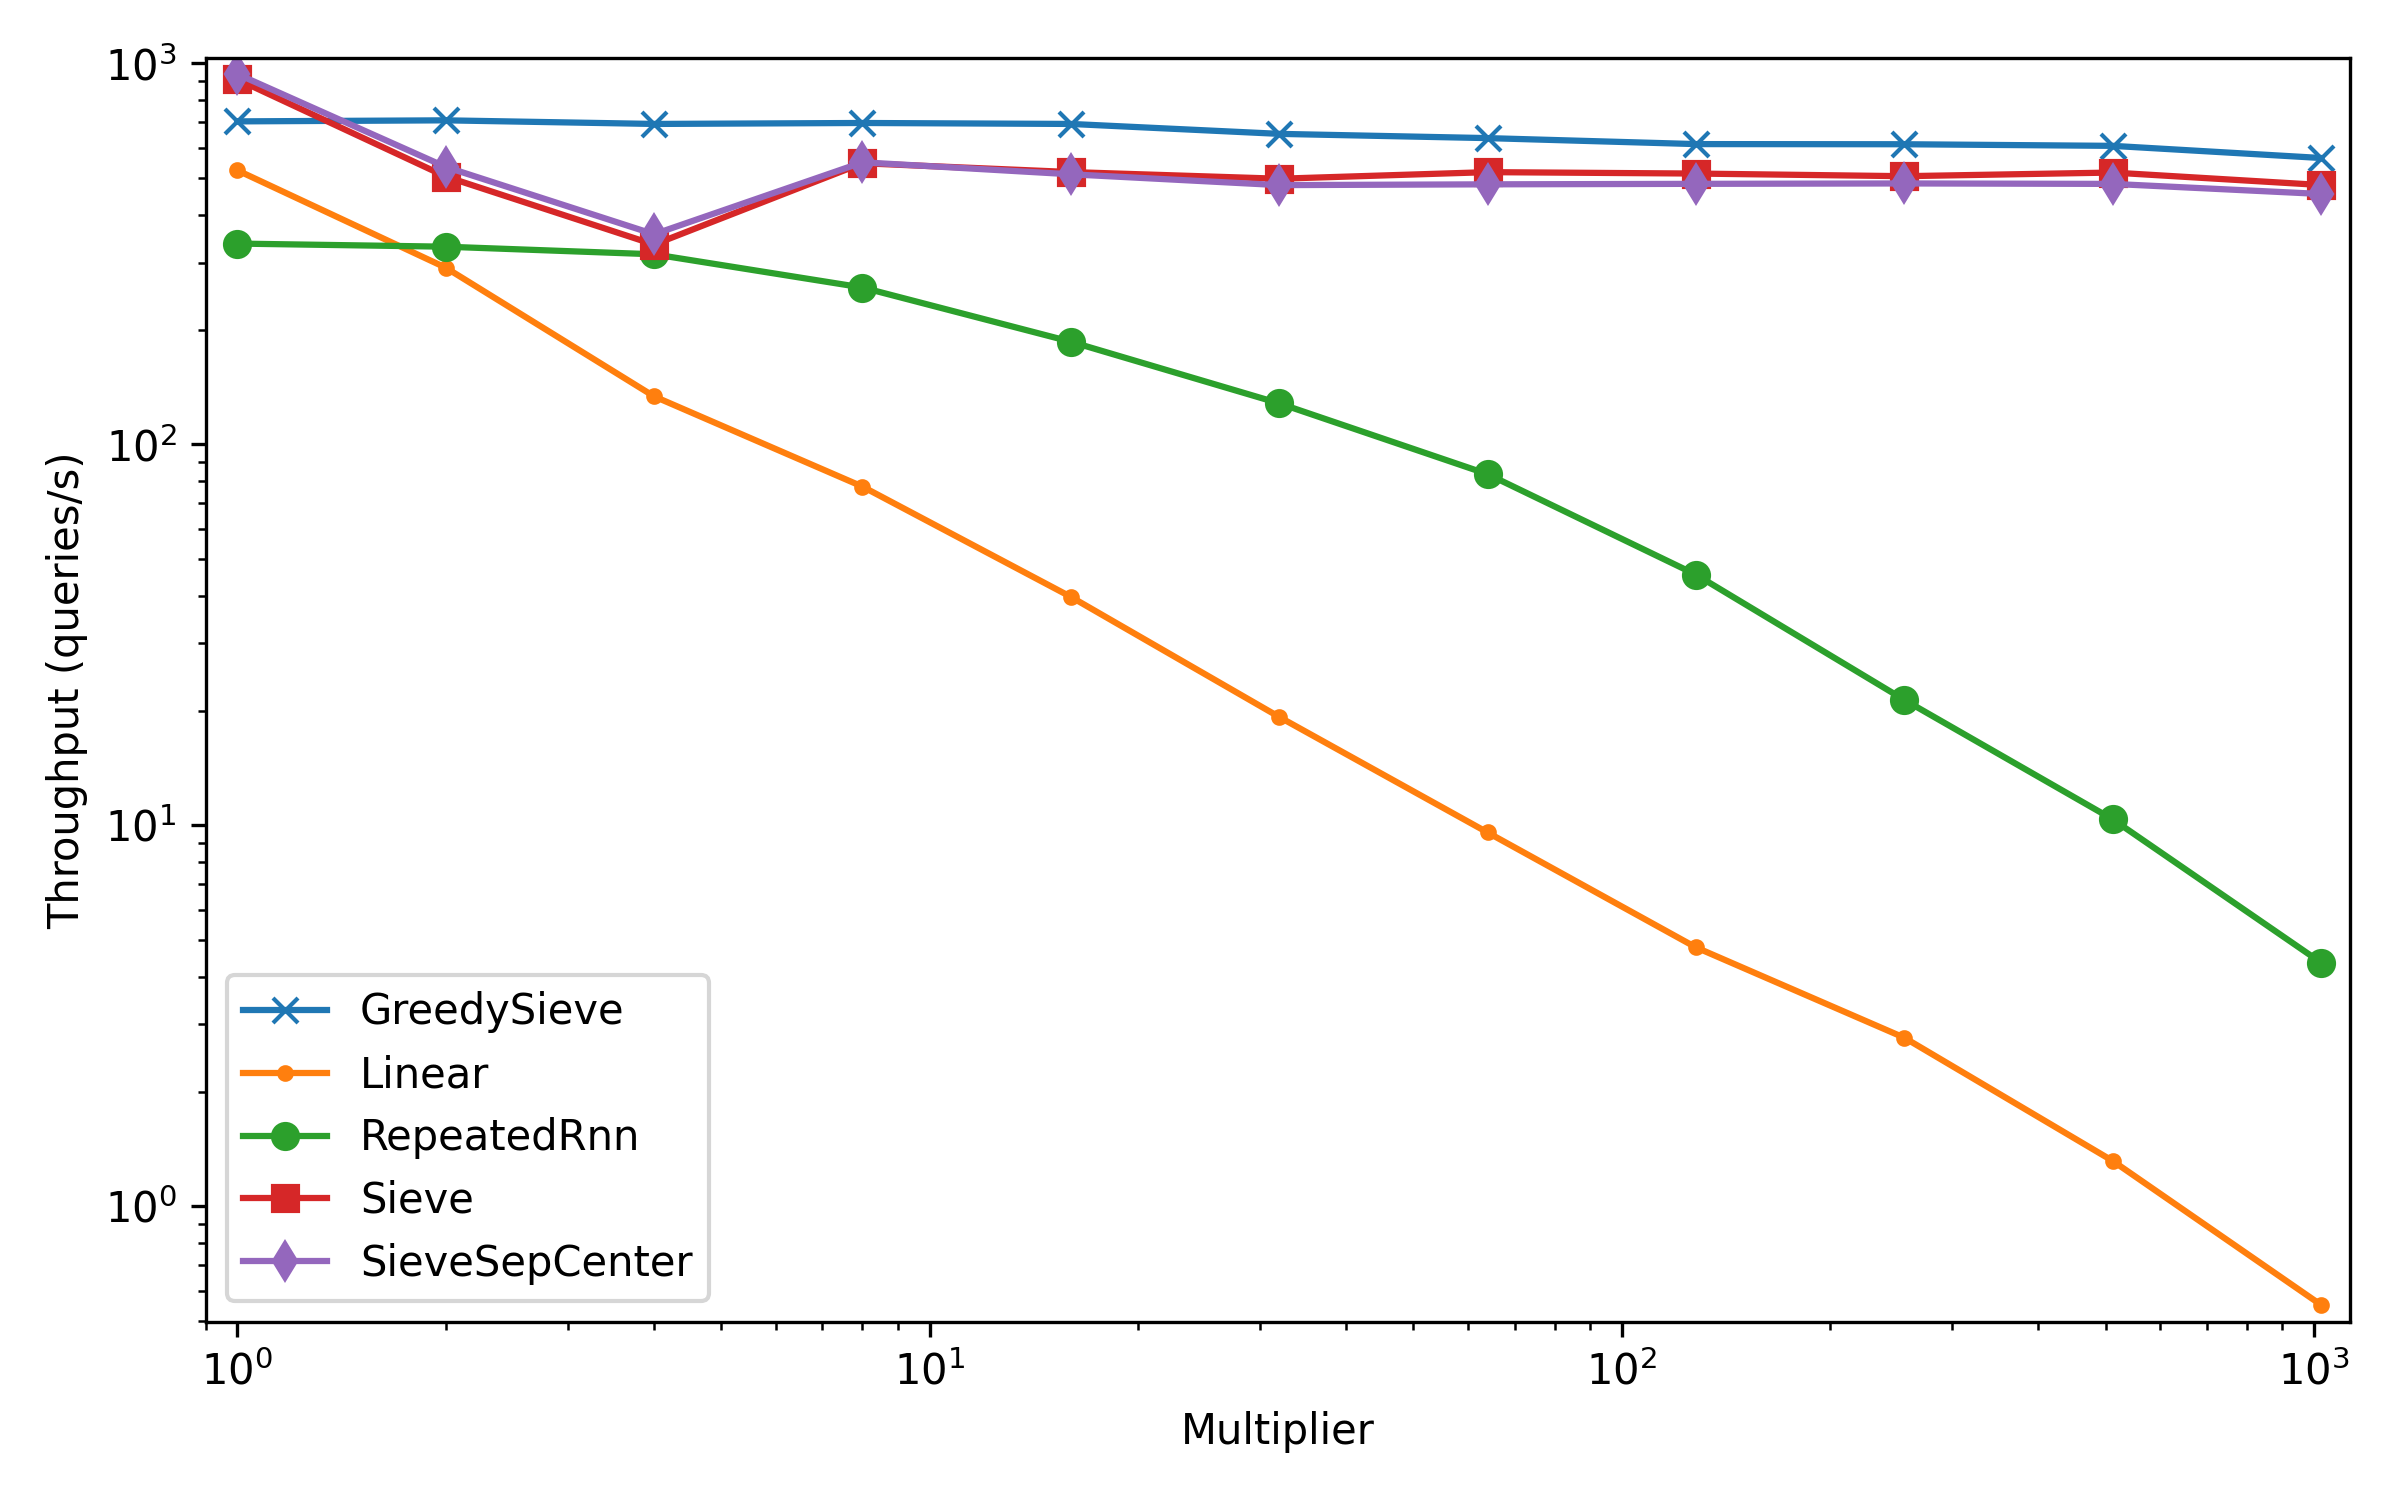
\includegraphics[width=3.4in]{images/result_plots/fashion-mnist_10_scaling.png}
    \caption{
        Fashion-mnist Scaling
    }
    \label{fig:results:fashion-mnist-scaling}
\end{figure}

% \begin{figure}[ht!]
%     \centering
%     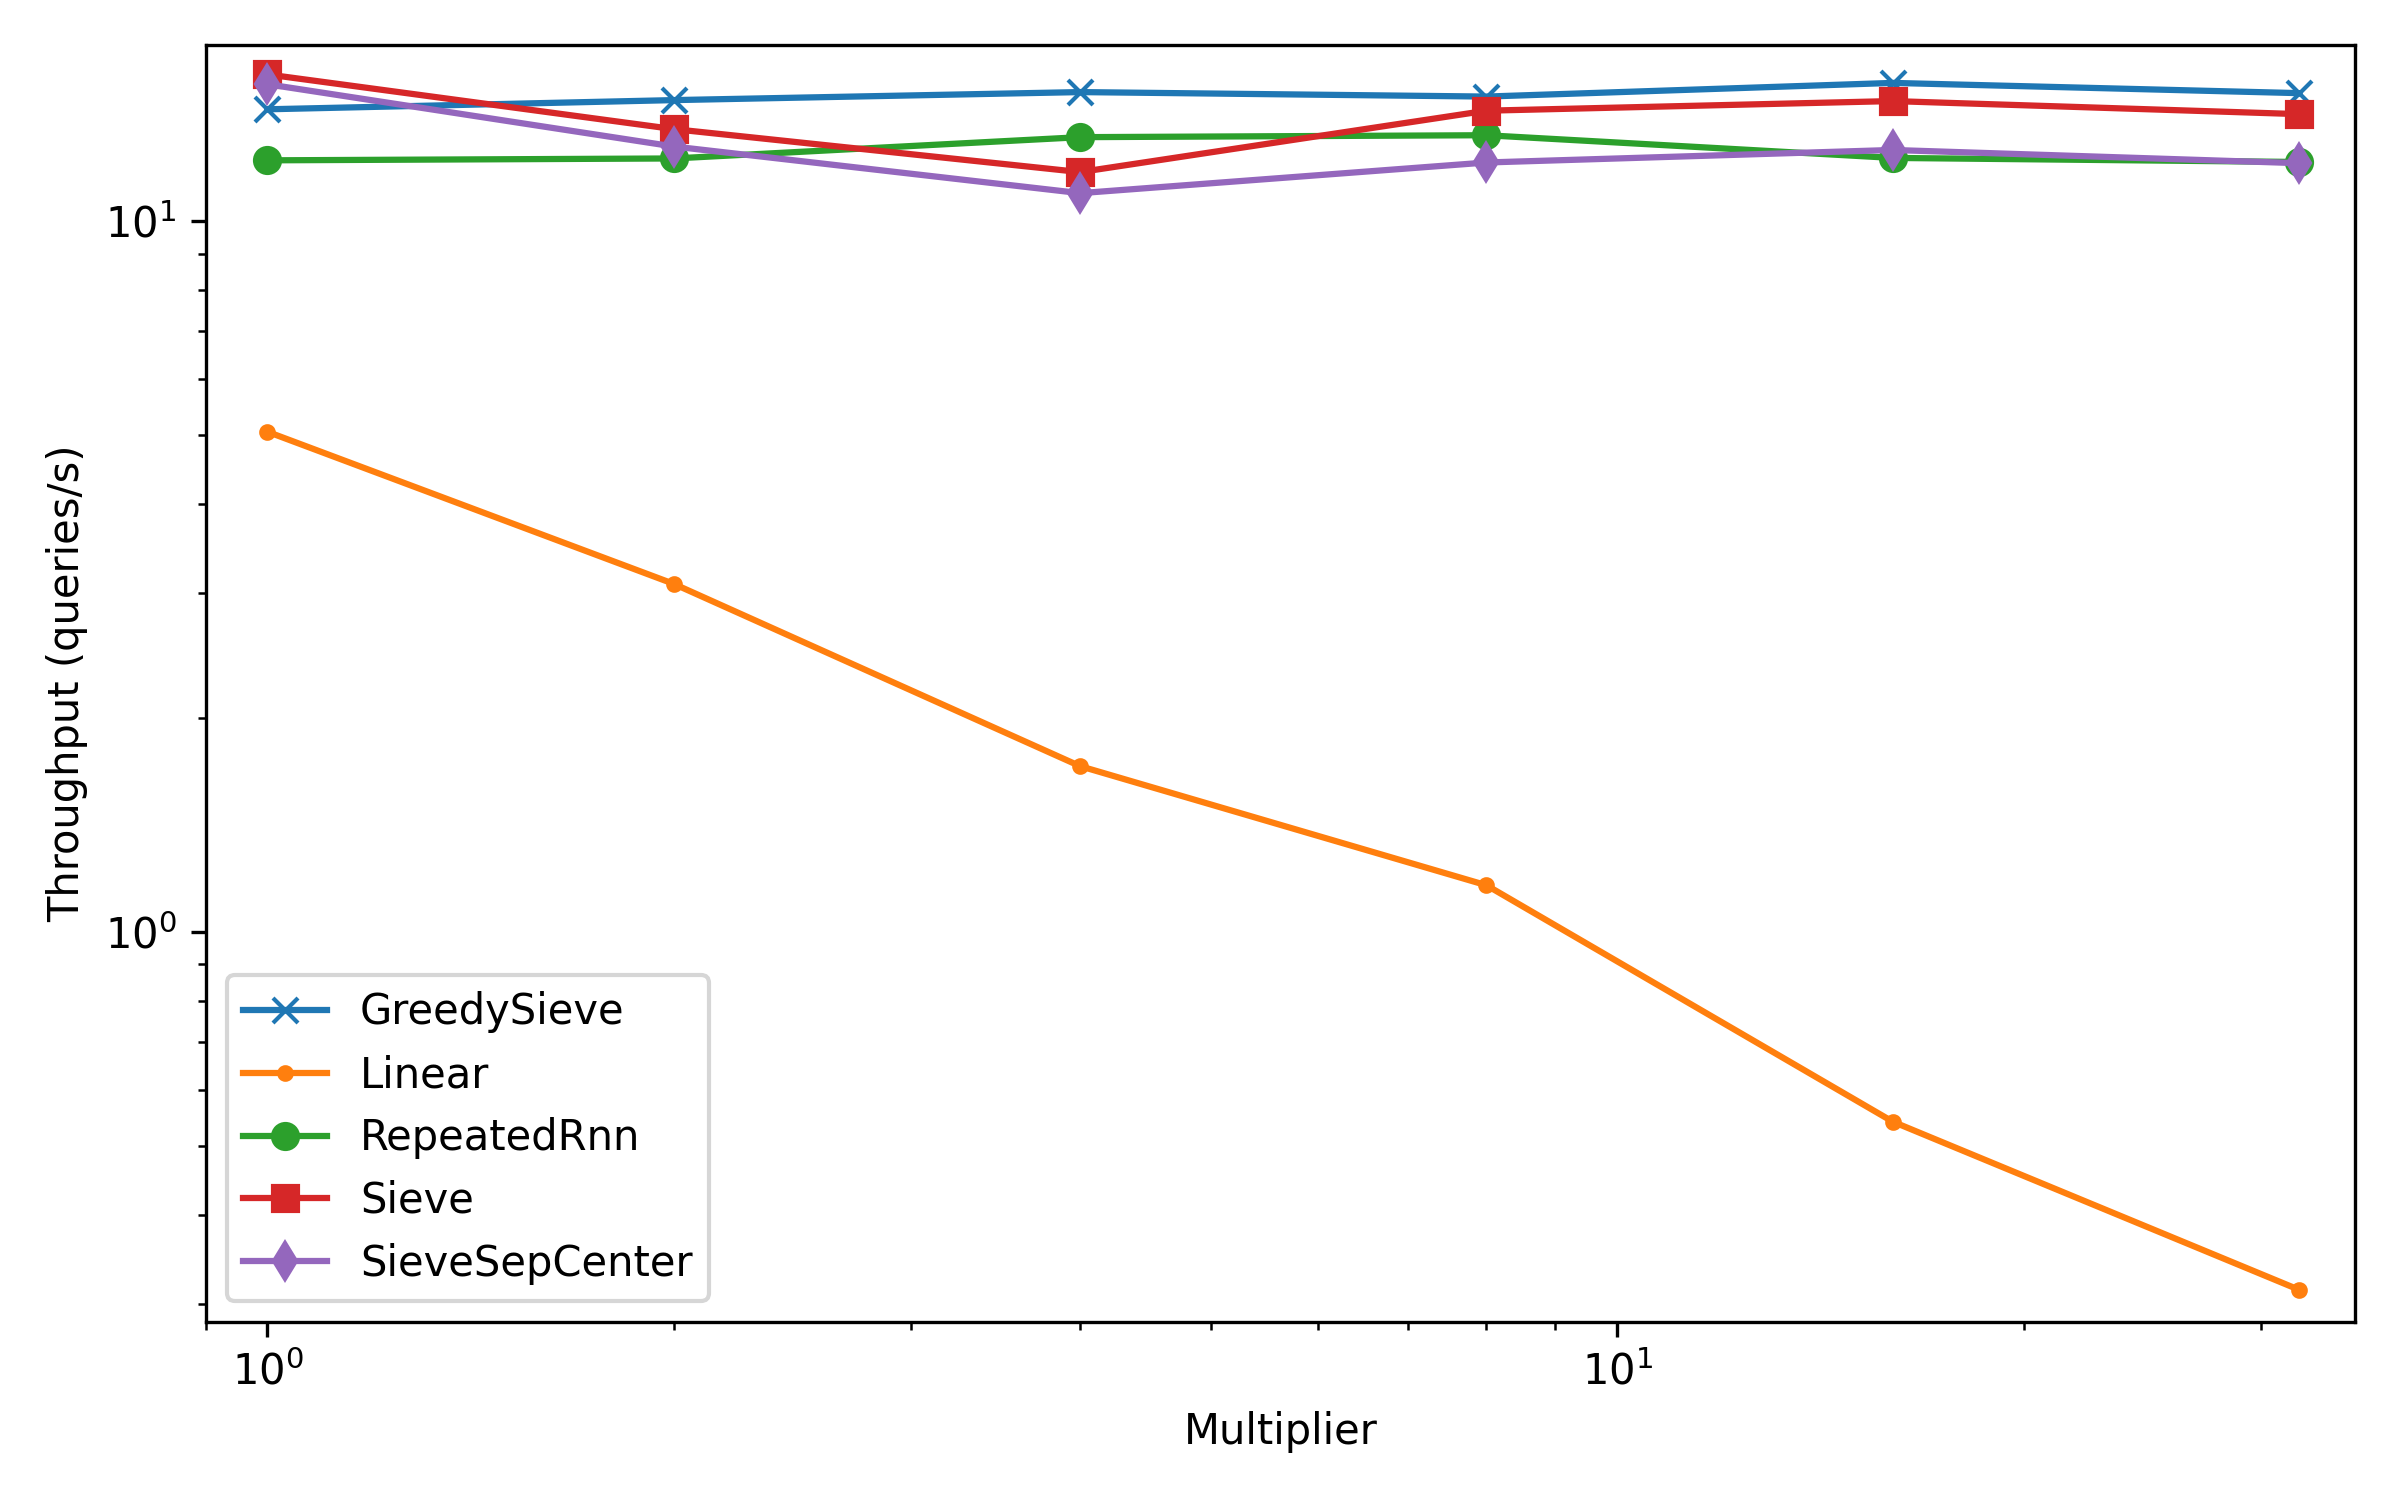
\includegraphics[width=3.4in]{images/result_plots/deep-image_10_scaling.png}
%     \caption{
%         Deep-image Scaling
%     }
%     \label{fig:results:deep-image-scaling}
% \end{figure}


\begin{figure}[ht!]
    \centering
    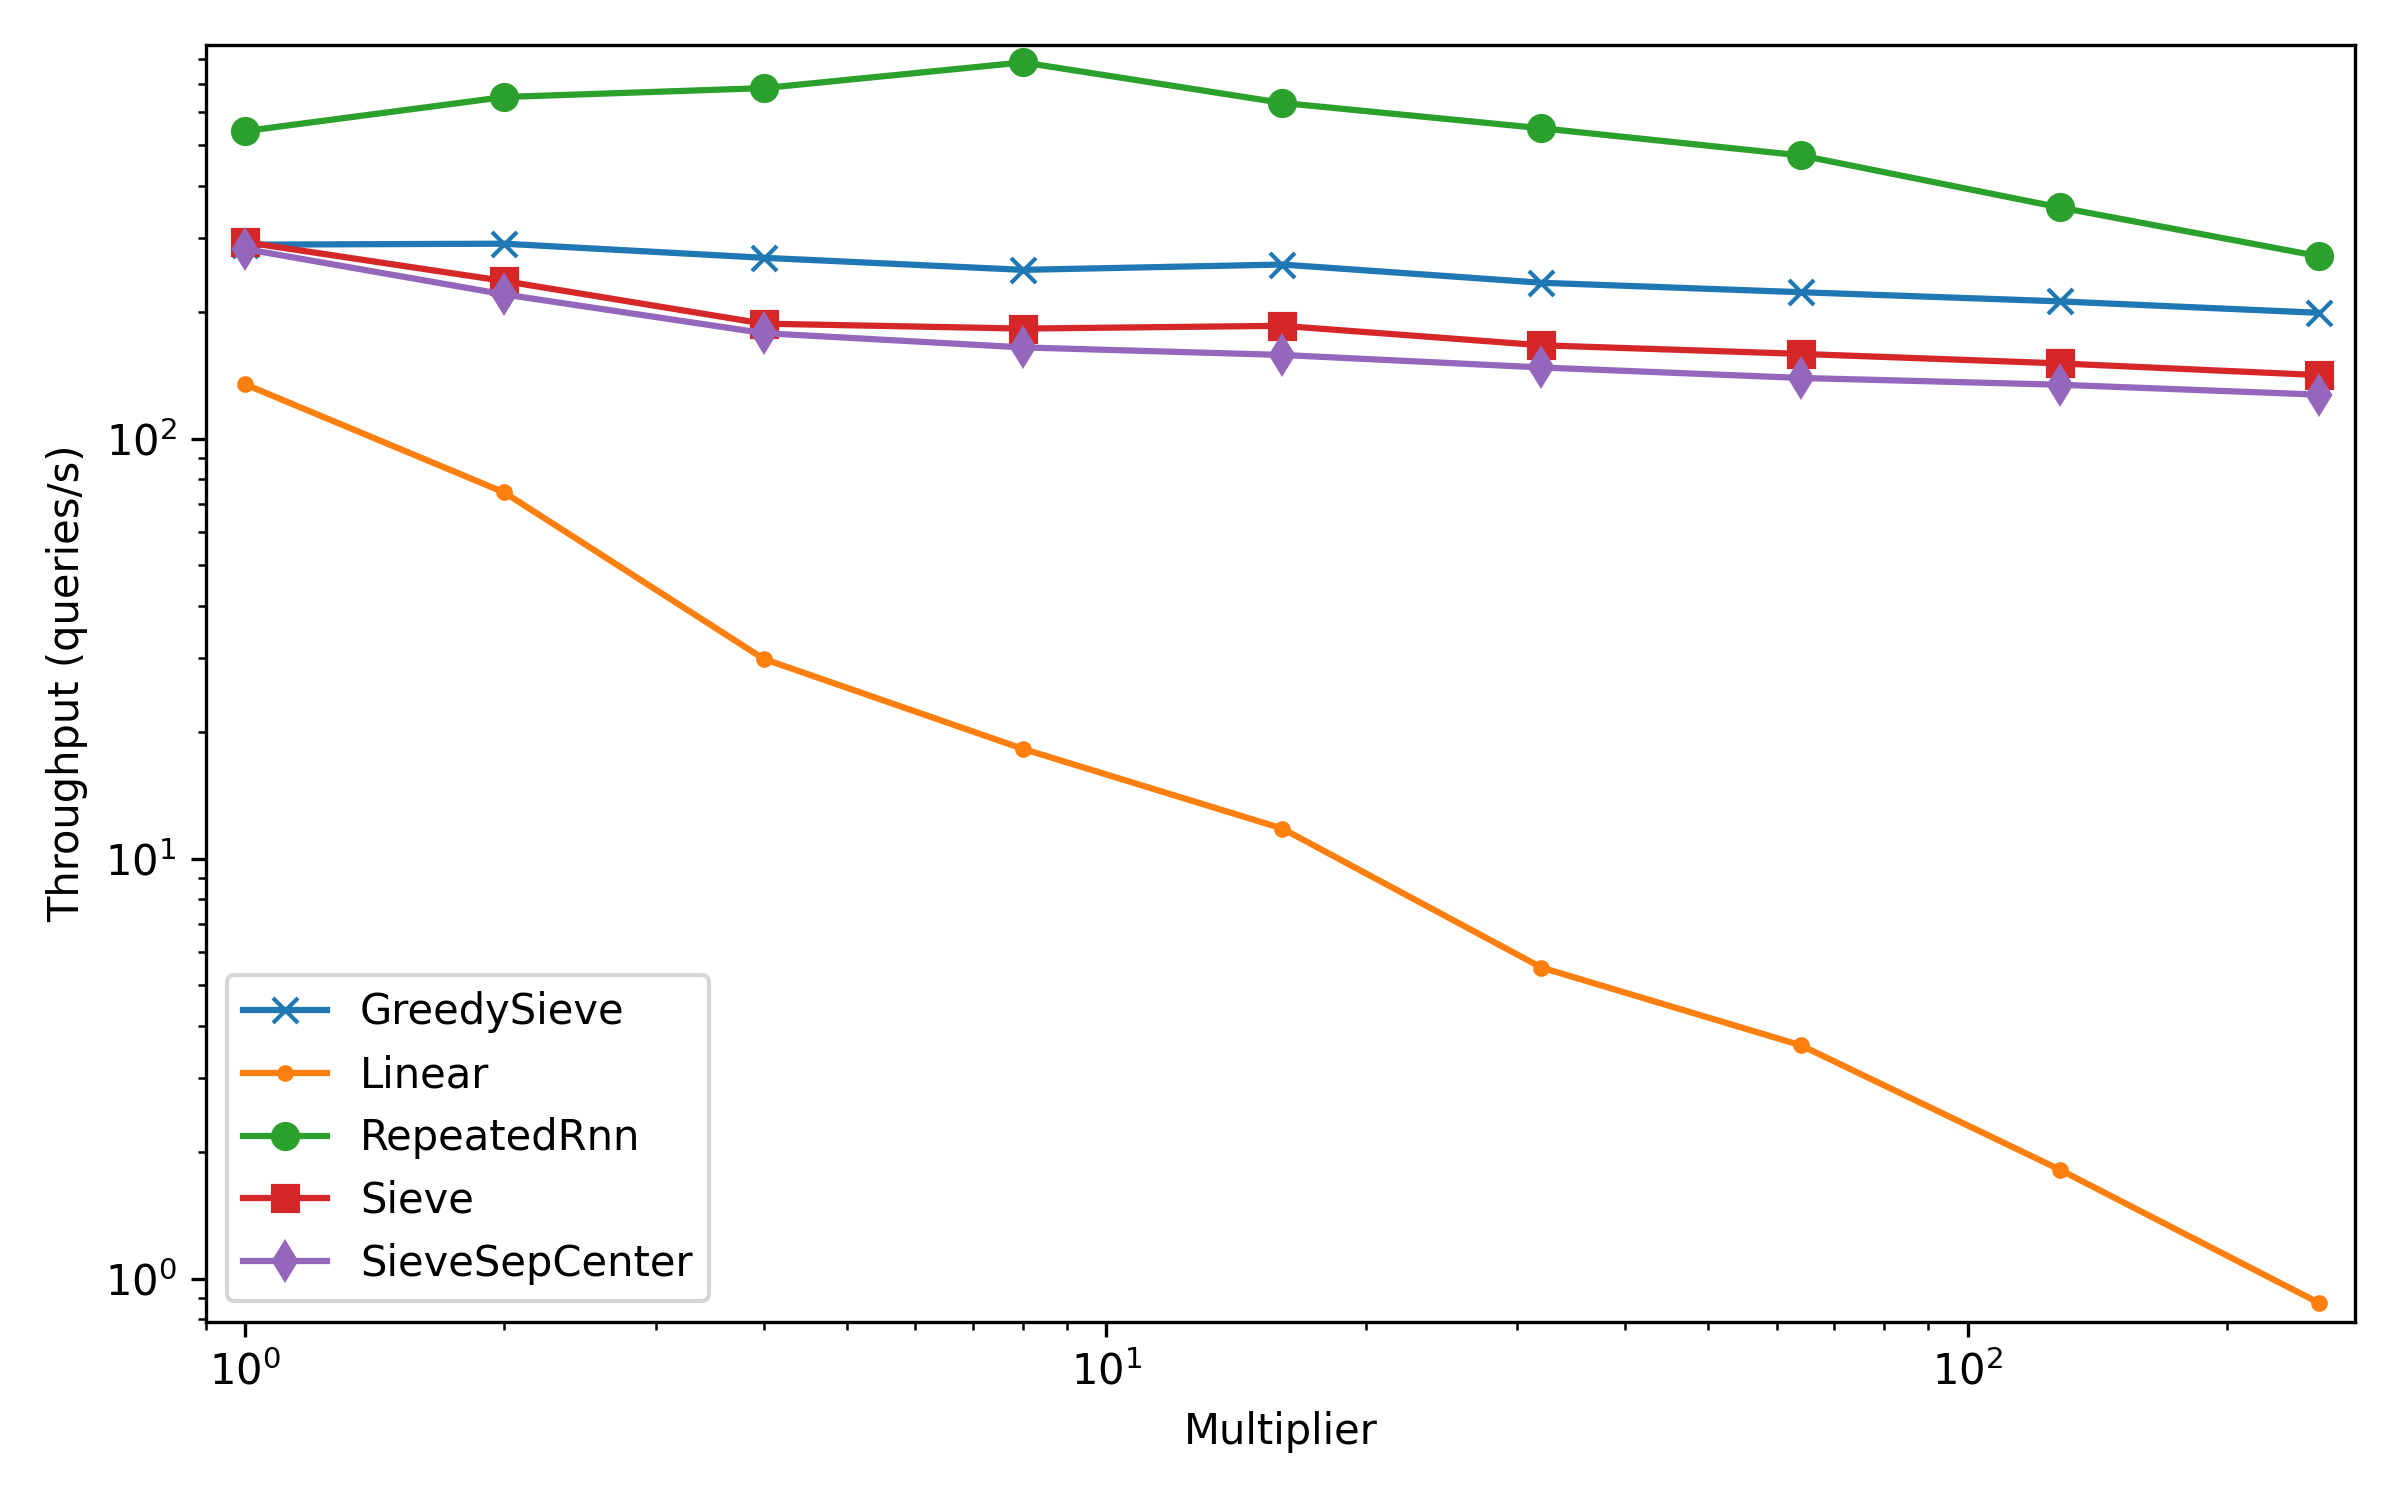
\includegraphics[width=3.4in]{images/result_plots/glove-25_10_scaling.png}
    \caption{
        Glove-25 Scaling
    }
    \label{fig:results:glove-25-scaling}
\end{figure}


\begin{figure}[ht!]
    \centering
    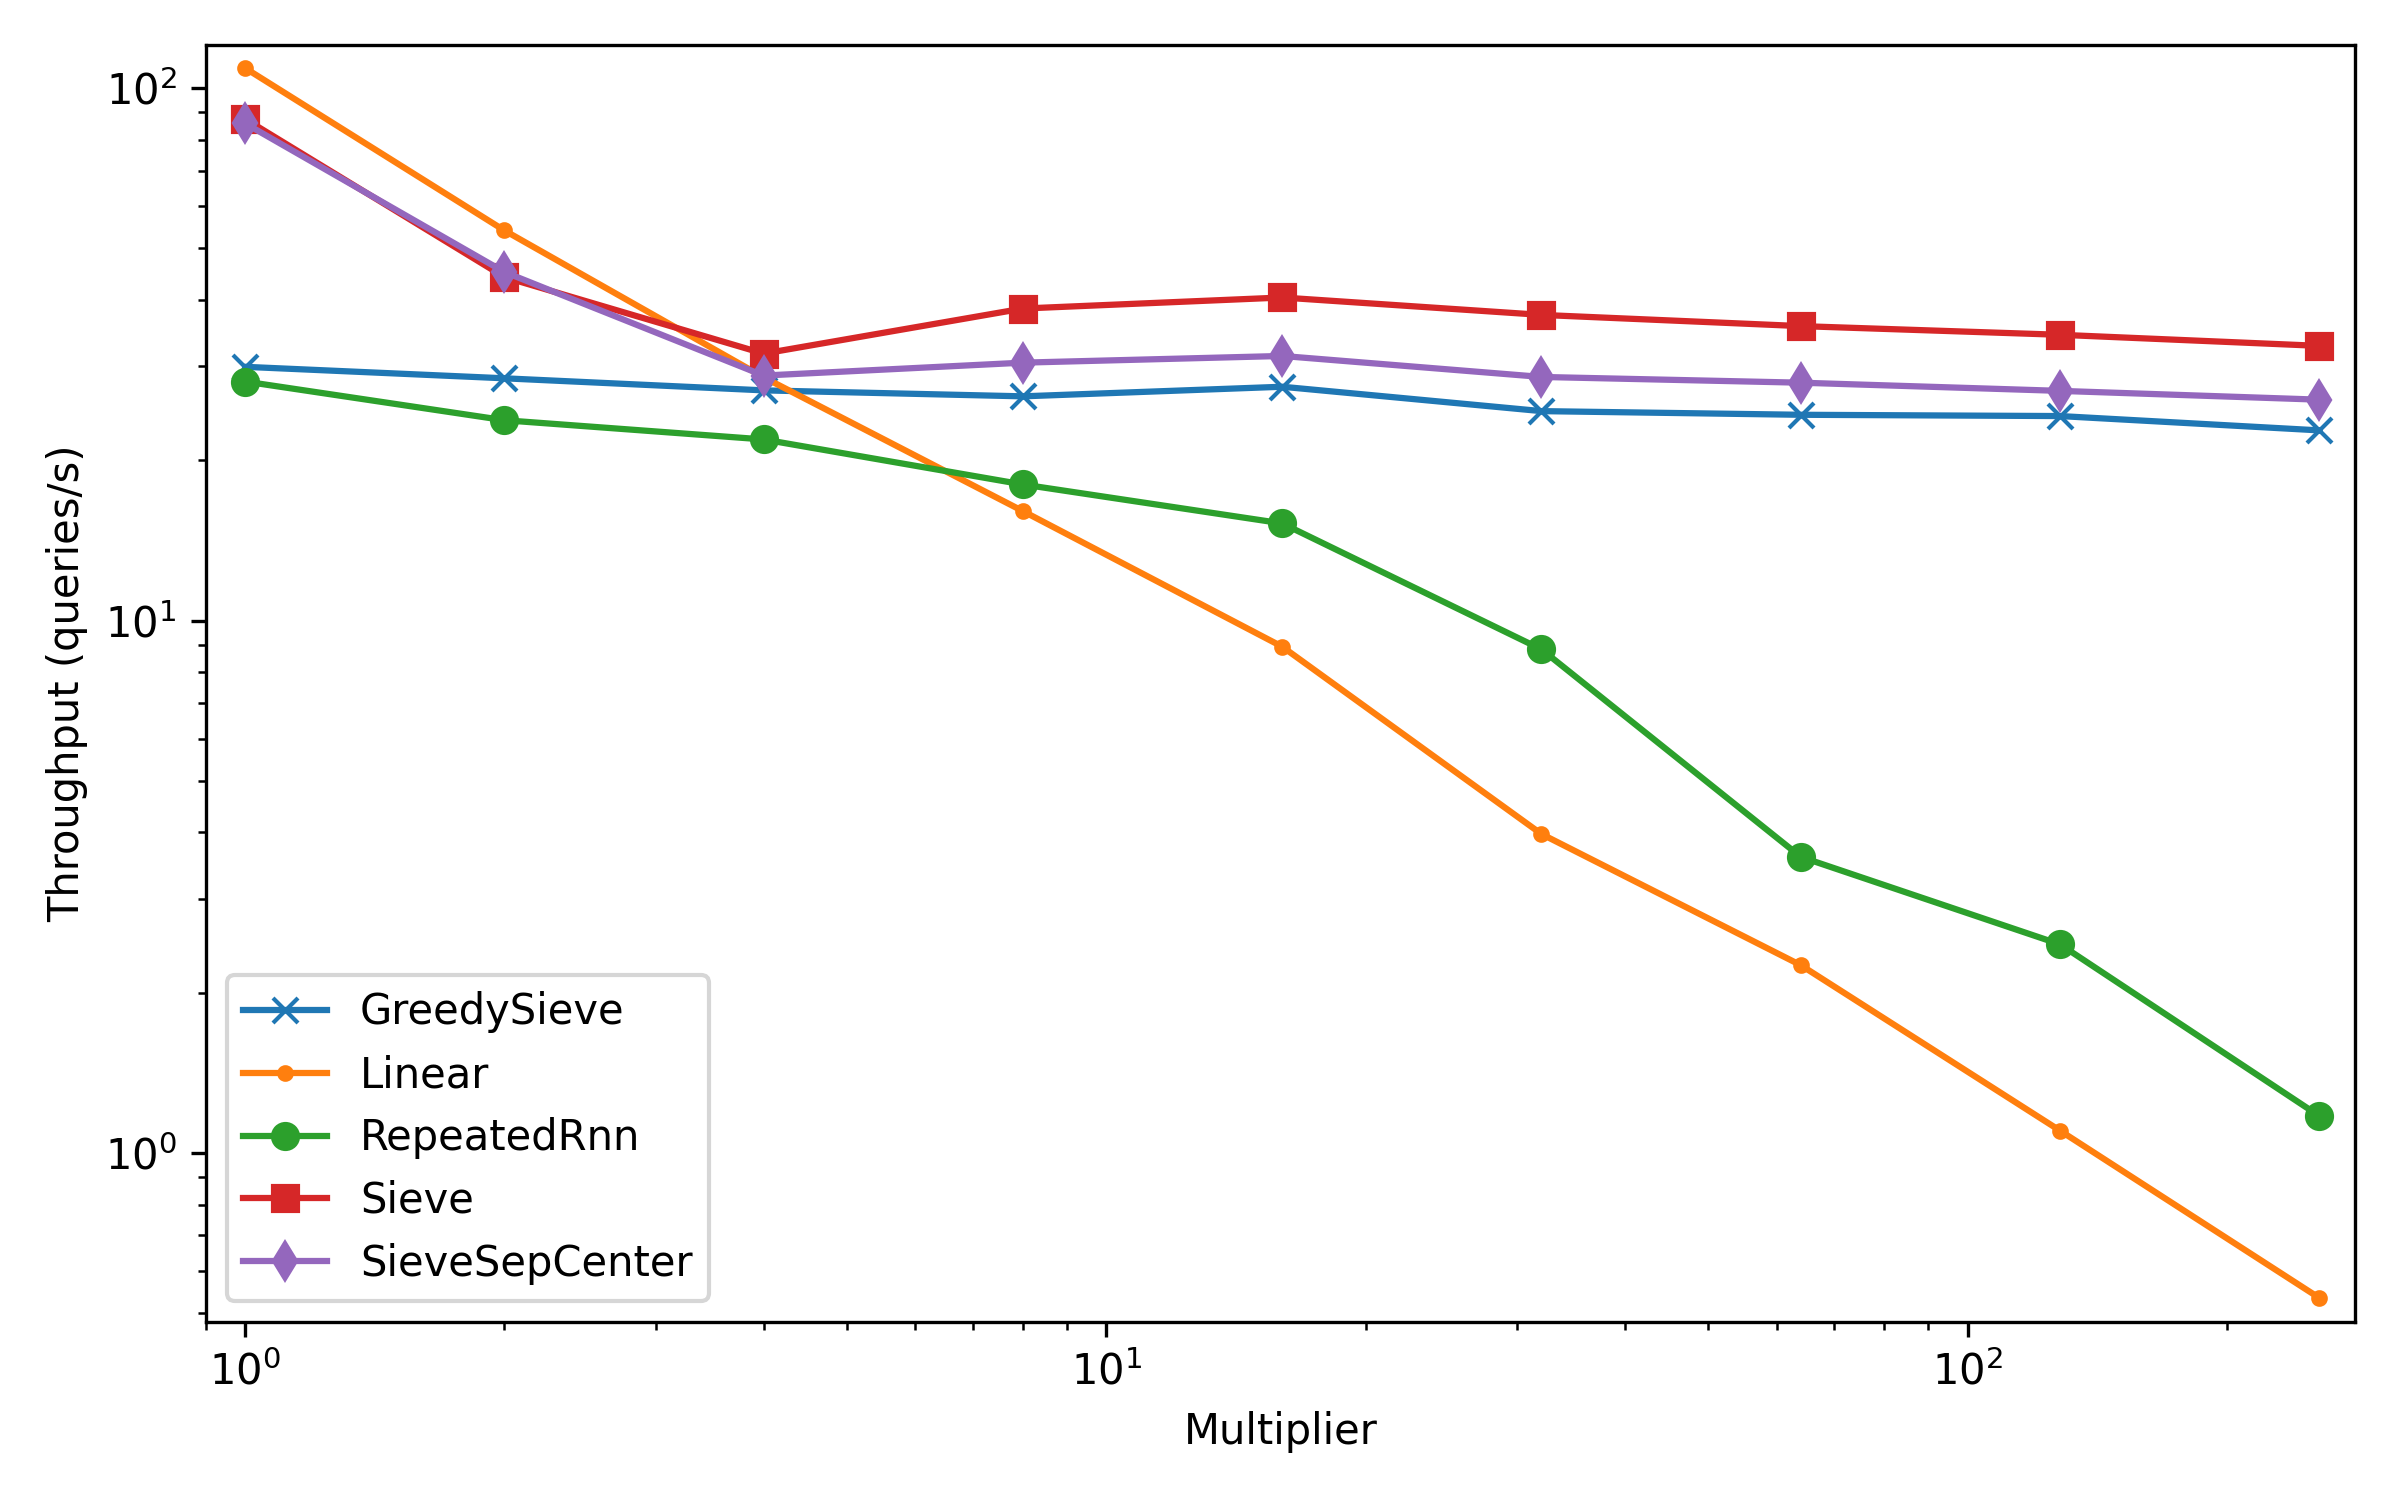
\includegraphics[width=3.4in]{images/result_plots/sift_10_scaling.png}
    \caption{
        Sift Scaling
    }
    \label{fig:results:sift-scaling}
\end{figure}

% We need to redo this plot so that we do not actually augment random datasets but instead take larger and larger 
% random datasets

\begin{figure}[ht!]
    \centering
    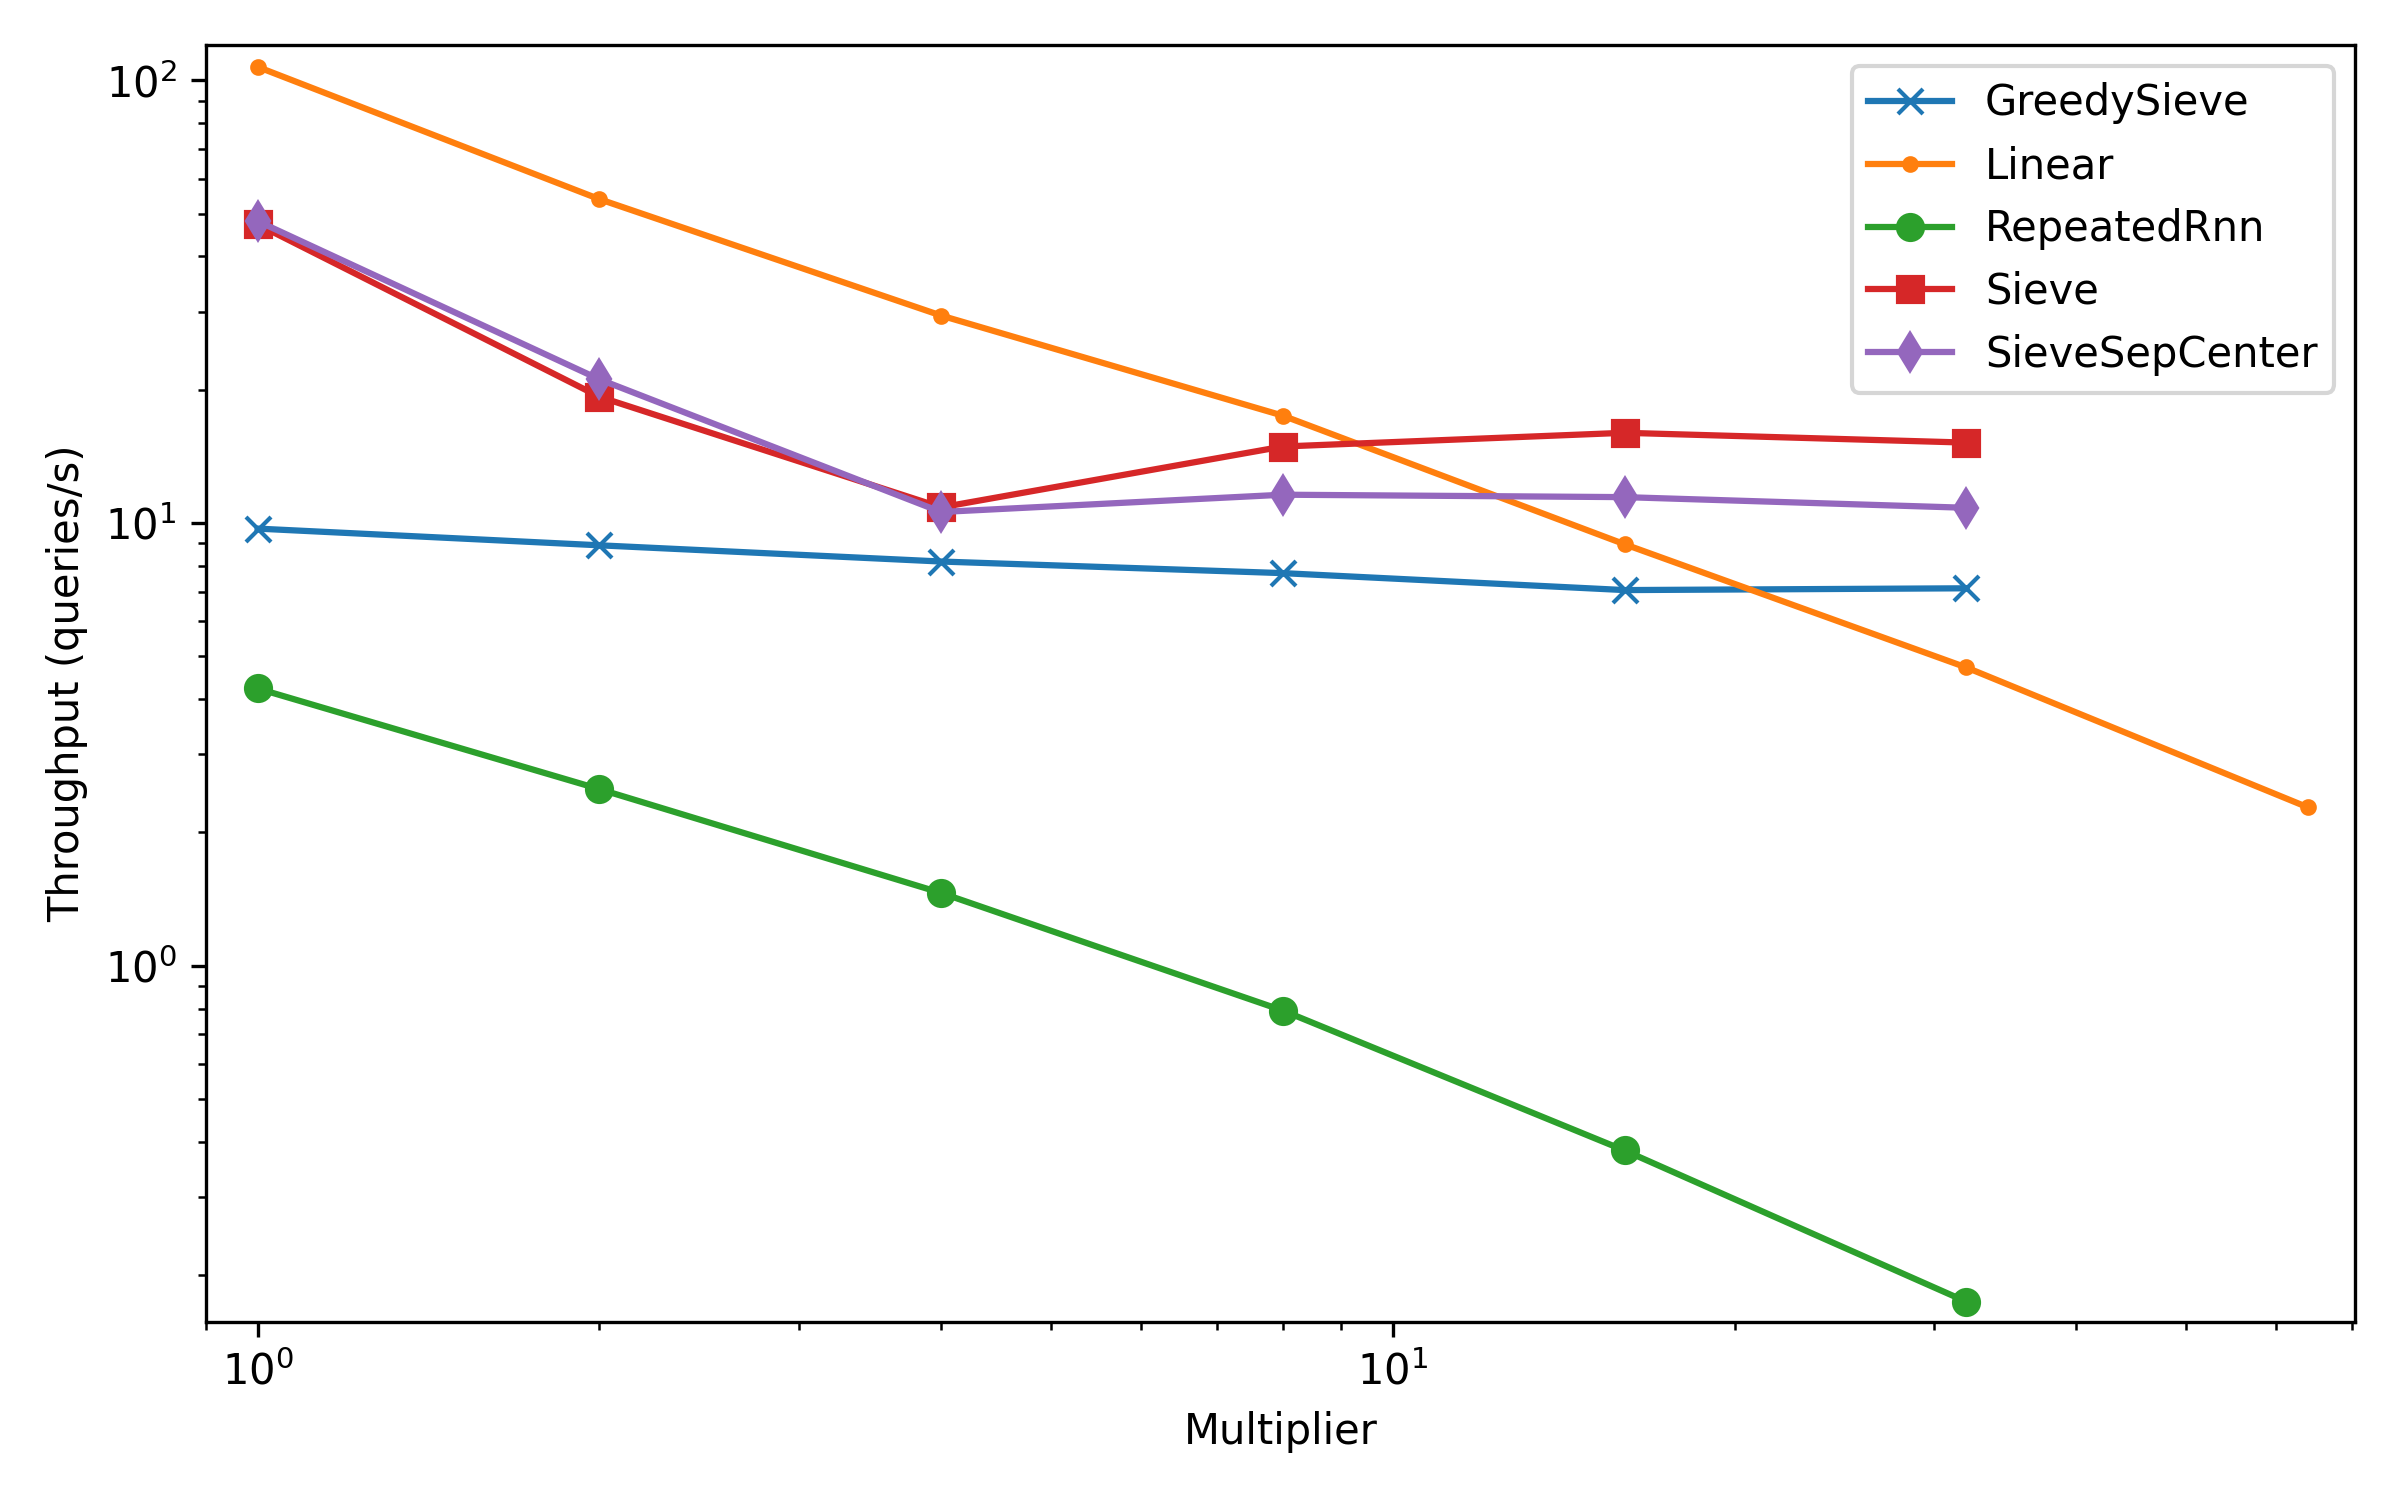
\includegraphics[width=3.4in]{images/result_plots/random_placeholder_10_scaling.png}
    \caption{
        Random Scaling
    }
    \label{fig:results:random-scaling}
\end{figure}


% We did not run any of the competitor's algorithms.
% We lifted the reported numbers from the ann-benchmarks site and their interactive plots.
% We made sure to use the same AWS instance as they did so it is a fair comparison.

% Tables \ref{table:results:ann-10} and \ref{table:results:ann-100} show the results of our benchmarks against FAISS, bruteforce-blas, and HNSW.
% The throughput values for these algorithms comes from the ANN benchmarks website's interactive plots, from which we can assess the throughput of each algorithm at a given recall value.

% We report the highest throughput value for each algorithm at a recall value of 1.0.
% We report the mean and median speedup factor of CAKES over each algorithm.
% For $k= 10$, we report a mean $7,654 \times$ (median $1,200 \times$) speedup over faiss-ivf, a mean $11,325 \times$ (median $2,821 \times$) speedup over bruteforce-blas, and a mean $485 \times$ (median $417 \times$) speedup over HNSW. 
% For $k=100$, we report a mean $4,479 \times$ (median $3,456 \times$) speedup over faiss-ivf, a mean $16,010 \times$ (median $13,548 \times$) speedup over bruteforce-blas, and a mean $403 \times$ (median $372 \times$) speedup over HNSW.

% For all datasets benchmarked in this manuscript, the auto-tuning method selected repeated $\rho$-nearest neighbor (Section~\ref{subsubsec:methods:knn-search:repeated-rnn}).

% We note that the mean and median speedup factors differ significantly for all methods, which suggests that the speedup factor is heavily dataset-dependent;
% in particular, across all algorithms, and both values of $k$, CAKES exhibits particularly high speedup factors with SIFT and GIST, under Euclidean distance.
% As GIST was designed to be a difficult dataset for classifiers~\cite{Lee2019PracticalLP}, CAKES's strong performance with this dataset is particularly encouraging.
% Further investigation of CAKES's performance on other challenging or adversarial datasets is warranted. 


\begin{table*}[!t]
    % \renewcommand{\arraystretch}{1.15}
    \caption{Runtime performance (queries per second) and recall of CAKES vs. other methods on the sift dataset. We use 1.000* to denote that the recall is imperfect, but rounds to 1.000 when we consider only three decimal places.}
    \label{table:results:ann-fashion}
    \vskip 0.15in
    \begin{center}
        \begin{small}
            \begin{sc}
                \begin{tabular}{|l|p{1cm}|p{1cm}|p{1cm}|p{1cm}|p{1cm}|p{1cm}|p{1cm}|p{1cm}|}
                    \hline
                    \textbf{Scaling Factor}  & \multicolumn{2}{|c|}{\textbf{annoy}} & \multicolumn{2}{|c|}{\textbf{faiss-flat}} & \multicolumn{2}{|c|}{\textbf{faiss-ivf-flat}}  & \multicolumn{2}{|c|}{\textbf{CAKES}} \\
                    \hline
                    &             QPS & Recall        & QPS & Recall      & QPS & Recall       & QPS & Recall       \\
                    \hline
                    1.000 & 2191.849 & 0.950 & 212.602 & 1.000 & 2009.483 & 1.000 & 2167.365 & 1.000 \\
                    \hline
                    2.000 & 2118.513 & 0.927 & 106.372 & 1.000 & 939.169 & 1.000* & 1141.225 & 1.000 \\
                    \hline
                    4.000 & 2043.628 & 0.898 & 53.077 & 1.000 & 461.016 & 0.997 & 982.117 & 1.000 \\
                    \hline
                    8.000 & 1925.593 & 0.857 & 26.577 & 1.000 & 225.827 & 0.995 & 1179.813 & 1.000 \\
                    \hline
                    16.000 & 1841.863 & 0.862 & 13.292 & 1.000 & 116.960 & 0.991 & 1201.409 & 1.000 \\
                    \hline
                    32.000 & 1850.943 & 0.775 & 6.647 & 1.000 & 59.148 & 0.985 & 1157.667 & 1.000 \\
                    \hline
                    64.000 & 1787.142 & 0.677 & 3.324 & 1.000 & 26.068 & 0.968 & 1102.849 & 1.000 \\
                    \hline
                    128.000 & 1659.660 & 0.538 & 1.662 & 1.000 & 13.265 & 0.964 & 1039.607 & 1.000 \\
                    \hline
                    256.000 & 1597.264 & 0.592 & 0.831 & 1.000 & 6.650 & 0.962 & 1058.972 & 1.000 \\
                    \hline
                    512.000 & 1826.362 & 0.581 & 0.416 & 1.000 & 3.563 & 0.949 & 1035.260 & 1.000 \\
                    \hline
                \end{tabular}
            \end{sc}
        \end{small}
    \end{center}
    \vskip -0.1in
\end{table*}





\begin{table*}[!t]
    % \renewcommand{\arraystretch}{1.15}
    \caption{Runtime performance (queries per second) and recall of CAKES vs. other methods on the fashion-mnist dataset. We use 1.000* to denote that the recall is imperfect, but rounds to 1.000 when we consider only three decimal places.}
    \label{table:results:ann-fashion}
    \vskip 0.15in
    \begin{center}
        \begin{small}
            \begin{sc}
                \begin{tabular}{|l|p{1cm}|p{1cm}|p{1cm}|p{1cm}|p{1cm}|p{1cm}|p{1cm}|p{1cm}|}
                    \hline
                    \textbf{Scaling Factor}  & \multicolumn{2}{|c|}{\textbf{annoy}} & \multicolumn{2}{|c|}{\textbf{faiss-flat}} & \multicolumn{2}{|c|}{\textbf{faiss-ivf-flat}}  & \multicolumn{2}{|c|}{\textbf{CAKES}} \\
                    \hline
                    &             QPS & Recall        & QPS & Recall      & QPS & Recall       & QPS & Recall       \\
                    \hline
                    1.000 & 2191.849 & 0.950 & 212.602 & 1.000 & 2009.483 & 1.000 & 2167.365 & 1.000 \\
                    \hline
                    2.000 & 2118.513 & 0.927 & 106.372 & 1.000 & 939.169 & 1.000* & 1141.225 & 1.000 \\
                    \hline
                    4.000 & 2043.628 & 0.898 & 53.077 & 1.000 & 461.016 & 0.997 & 982.117 & 1.000 \\
                    \hline
                    8.000 & 1925.593 & 0.857 & 26.577 & 1.000 & 225.827 & 0.995 & 1179.813 & 1.000 \\
                    \hline
                    16.000 & 1841.863 & 0.862 & 13.292 & 1.000 & 116.960 & 0.991 & 1201.409 & 1.000 \\
                    \hline
                    32.000 & 1850.943 & 0.775 & 6.647 & 1.000 & 59.148 & 0.985 & 1157.667 & 1.000 \\
                    \hline
                    64.000 & 1787.142 & 0.677 & 3.324 & 1.000 & 26.068 & 0.968 & 1102.849 & 1.000 \\
                    \hline
                    128.000 & 1659.660 & 0.538 & 1.662 & 1.000 & 13.265 & 0.964 & 1039.607 & 1.000 \\
                    \hline
                    256.000 & 1597.264 & 0.592 & 0.831 & 1.000 & 6.650 & 0.962 & 1058.972 & 1.000 \\
                    \hline
                    512.000 & 1826.362 & 0.581 & 0.416 & 1.000 & 3.563 & 0.949 & 1035.260 & 1.000 \\
                    \hline
                \end{tabular}
            \end{sc}
        \end{small}
    \end{center}
    \vskip -0.1in
\end{table*}

% \begin{table*}[!t]
%     % \renewcommand{\arraystretch}{1.15}
%     \caption{Runtime performance (queries per second) of CAKES and Speedup Factor over Naive Linear Search, $k=10$}
%     \label{table:results:ann-alt-10}
%     \vskip 0.15in
%     \begin{center}
%         \begin{small}
%             \begin{sc}
%                 \begin{tabular}{|l|l|l|l|l|}
%                     \hline
%                     \textbf{Dataset} & \textbf{CAKES Throughput} & \textbf{Speedup Factor over Linear} \\
%                     \hline
%                     deep-image       & 232.1                     & 37.2      \\
%                     \hline
%                     mnist            & 129,300                   & 101.9      \\
%                     \hline
%                     glove-50         & 10,950                    & 12.28      \\
%                     \hline 
%                     glove-200        & 2,290                     & 8.55     \\
%                     \hline
%                     lastfm           & 13,950                    & 4.55           \\
%                     \hline
%                 \end{tabular}
%             \end{sc}
%         \end{small}
%     \end{center}
%     \vskip -0.1in
% \end{table*}


% \begin{table*}[!t]
%     % \renewcommand{\arraystretch}{1.15}
%     \caption{Runtime performance (queries per second) of CAKES and Speedup Factor over Naive Linear Search, $k=100$}
%     \label{table:results:ann-alt-100}
%     \vskip 0.15in
%     \begin{center}
%         \begin{small}
%             \begin{sc}
%                 \begin{tabular}{|l|l|l|l|l|l|}
%                     \hline
%                     \textbf{Dataset} & \textbf{CAKES Throughput} & \textbf{Speedup Factor over Linear} \\
%                     \hline
%                     deep-image        & 157.3                    & 25.74                               \\                            
%                     \hline
%                     mnist             & 71,090                   & 56.63                               \\
%                     \hline
%                     glove-50          & 8,867                    & 9.84                                \\
%                     \hline 
%                     glove-200         & 2,264                    & 8.49                                \\
%                     \hline
%                     lastfm            & 13,950                   & 4.55                                \\
%                     \hline
%                 \end{tabular}
%             \end{sc}
%         \end{small}
%     \end{center}
%     \vskip -0.1in
% \end{table*}
